%~~~~~~~~~~~~~~~~~~~~~~~~~~~~~~~~~~~~~~~~~~~~%
\begin{frame}[plain,noframenumbering]
    \titlepage
\end{frame}
%~~~~~~~~~~~~~~~~~~~~~~~~~~~~~~~~~~~~~~~~~~~~%
\begin{frame}[c]{Lecture format}
    \begin{center}
        \begin{tikzpicture}
            \foreach \f [count=\n from 0] in {Calendar, Time, Placeholder, Person, Newsletter}{
                \begin{scope}
                    \clip (0,-1.5*\n) circle[radius=5mm];
                    \node (A\n) at (0,-1.5*\n) {\includegraphics[width=10mm]{\f}};
                \end{scope}
            }
            \node[right = of A0] {\{07,08,09\}.10.2019};
            \node[right = of A1] {Morning: 09:15 to 12:00$\quad$ Afternoon: 14:15 to 17:00};
            \node[right = of A2] {Always at ITP, room 02.116};
            \node[right = of A3] {Dr. Alessandro Sciarra};
            \node[right = of A4] {sciarra@th.physik.uni-frankfurt.de};
        \end{tikzpicture}
    \end{center}
\end{frame}
%~~~~~~~~~~~~~~~~~~~~~~~~~~~~~~~~~~~~~~~~~~~~%
\begin{frame}{Who am I?}
    \begin{varblock}{quote}[0.68\textwidth]{Ancient popular wisdom}
        \guillemotleft{}I am not saying to be Superman, I am just saying nobody has ever seen me and Superman together in the same room.\guillemotright
    \end{varblock}
    \vspace{5mm}
    \begin{itemize}
        \item Member of the Software Development Center \\ $\to\;$ Z02 project of the CRC-TR211 collaboration
        \item A ``lattice practitioner''
        \item A dreamer who flatters himself that
              \begin{itemize}
                  \item physicists will one day \PB{properly} use the IT tools they use
                  \item IT people will teach IT to physicists and work next to them
                  \item physicists will be able to focus on physics
              \end{itemize}
        \item Not really a bash guru, but rather a self-thought bash enthusiast
    \end{itemize}
    \begin{tikzpicture}[remember picture, overlay]
        \node[anchor=south east, inner sep=0] at (current page.south east) {
\includegraphics[height=4cm]{Superman}};
    \end{tikzpicture}
\end{frame}
%~~~~~~~~~~~~~~~~~~~~~~~~~~~~~~~~~~~~~~~~~~~~%
\begin{frame}{What is \URL[PP]{https://www.gnu.org/software/bash/}{Bash}?}
    \begin{tikzpicture}[remember picture, overlay]
        \node[anchor=north east] (logo) at ($(current page.north east)-(3mm,3mm)$) {
\includegraphics[width=25mm]{BashLogo}};
        \node[below = 1mm of logo.north east, anchor=east, font=\tiny] {\URL{https://commons.wikimedia.org/w/index.php?curid=53428398}{Bash logo}};
    \end{tikzpicture}
    \vspace{-3mm}
    \begin{itemize}
        \item Scripting/command language
        \item Unix shell $\;\leftrightarrow\;$ command processor
        \item First release in 1989, current version v5.0 (Jan 2019) $\quad\to\;$ \URL[PS]{http://ftp.gnu.org/gnu/bash/}{download Bash}
    \end{itemize}
    \begin{varblock}{quote}[0.9\textwidth]{GNU Bash}
        Bash is the GNU Project's shell.
        Bash is the Bourne Again SHell.
        Bash is an sh-compatible shell that incorporates useful features from the Korn shell (\textnormal{ksh}) and C shell (\textnormal{csh}).
        [\ldots]
        It offers functional improvements over \textnormal{sh} for both programming and interactive use.
        In addition, most \textnormal{sh} scripts can be run by Bash without modification.
    \end{varblock}
    \uncover<2>{
        \begin{itemize}
            \item A scripting language which may get hard to read $\to$ you need some \PP{``code sense''}
            \item The effort required to a newbie is quite large $\to$ you need to practice!
            \item \ldots{}I am here to help you filling up this gap!
        \end{itemize}
    }
\end{frame}
%~~~~~~~~~~~~~~~~~~~~~~~~~~~~~~~~~~~~~~~~~~~~%
\begin{frame}{Why should I know Bash?}
    
\end{frame}
%~~~~~~~~~~~~~~~~~~~~~~~~~~~~~~~~~~~~~~~~~~~~%
\begin{frame}{The mind setup of this course}
    
\end{frame}
%~~~~~~~~~~~~~~~~~~~~~~~~~~~~~~~~~~~~~~~~~~~~%
\begin{frame}{Notation}
    
\end{frame}
%~~~~~~~~~~~~~~~~~~~~~~~~~~~~~~~~~~~~~~~~~~~~%
\begin{frame}{What will we explore?}
    
\end{frame}
%~~~~~~~~~~~~~~~~~~~~~~~~~~~~~~~~~~~~~~~~~~~~%
\begin{frame}{Bonus track: Iceland}{The magic of an incredible island}
    \begin{tikzpicture}[remember picture, overlay]
        \node (plan) at ($(current page.center)-(0,6mm)$) {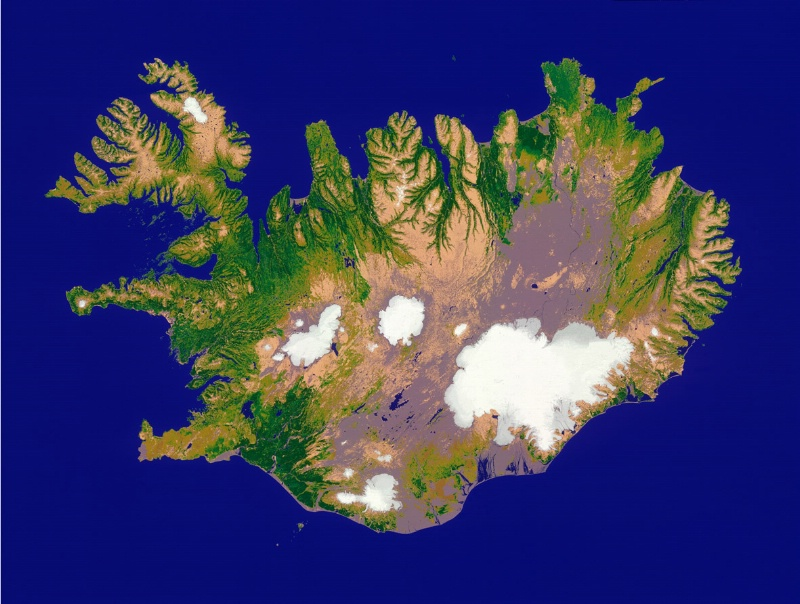
\includegraphics[width=0.8\textwidth, clip, trim=1mm 0 0 0]{Map2}};
        \begin{scope}[x={($ (plan.south east) - (plan.south west) $ )},y={( $ (plan.north west) - (plan.south west)$ )}, shift={(plan.south west)}]
            %\draw[help lines,xstep=.1,ystep=.1] (0,0) grid (1,1);
            \node[anchor=south, inner sep=0] at (0.25,0.32) {
\includegraphics[width=3mm]{Pin}};
            \node[anchor=south, inner sep=0] at (0.24,0.28) {
\includegraphics[width=3mm]{Pin}};
            \node[anchor=south, inner sep=0] at (0.31,0.34) {
\includegraphics[width=3mm]{Pin}};
            \node[anchor=south, inner sep=0] at (0.71,0.29) {
\includegraphics[width=3mm]{Pin}};
            \node[anchor=south, inner sep=0] at (0.47,0.14) {
\includegraphics[width=3mm]{Pin}};
        \end{scope}
    \end{tikzpicture}
\end{frame}
%~~~~~~~~~~~~~~~~~~~~~~~~~~~~~~~~~~~~~~~~~~~~%
\begin{frame}{A short but intense journey}
    
\end{frame}
%~~~~~~~~~~~~~~~~~~~~~~~~~~~~~~~~~~~~~~~~~~~~%